% \documentclass[table]{beamer}
\documentclass[table,handout]{beamer}
\setbeameroption{show notes}
% \setbeameroption{hide notes}
% \setbeameroption{show only notes}
\usepackage{varwidth}

\newif\ifhide
\newif\ifpost
\newif\ifhideclicker

% \hidetrue
% \hideclickertrue
% \posttrue

\newcommand{\whiteout}[1]{\textcolor{white}{#1}}
% \newcommand{\whiteoutbox}[1]{\fcolorbox{white}{white}{\parbox{\dimexpr \linewidth-2\fboxsep-2\fboxrule}{\whiteout{#1}}}}
% \newcommand{\notebox}[1]{\fcolorbox{blue}{white}{\parbox{\dimexpr \linewidth-2\fboxsep-2\fboxrule}{#1}}}
\newcommand{\whiteoutbox}[1]{\fcolorbox{white}{white}{\parbox{\linewidth}{\whiteout{#1}}}}
\newcommand{\notebox}[1]{\fcolorbox{blue}{white}{\parbox{\linewidth}{#1}}}
\newcommand{\blankbox}[1]{\phantom{\varwidth{\linewidth}\whiteoutbox{#1}\endvarwidth}}
\newcommand{\blank}[1]{\phantom{\varwidth{\linewidth}#1\endvarwidth}}

\ifhide%
    \newcommand{\hmask}[1]{\blank{#1}}%
\else%
    \newcommand{\hmask}[1]{#1}%
\fi

\ifhide%
    \newcommand{\wout}[1]{\whiteout{#1}}%
\else%
    \newcommand{\wout}[1]{#1}%
\fi

\ifhide%
    \newcommand{\hignore}[1]{}%
\else%
    \newcommand{\hignore}[1]{#1}%
\fi

\ifpost%
    \newcommand{\nopost}[1]{}%
\else%
    \newcommand{\nopost}[1]{#1}%
\fi

\ifhideclicker%
    \newcommand{\clickerslide}[1]{\stepcounter{clickerQuestionCounter}%
        \begin{frame}[t]
            \textcolor{blue}{Q \arabic{clickerQuestionCounter}:}
        \end{frame}}
\else%
    \newcommand{\clickerslide}[1]{#1}%
\fi

\ifhide%
    \newcommand{\hidebox}[1]{\blank{#1}}%
\else%
    \newcommand{\hidebox}[1]{\notebox{#1}}%
\fi

\ifhide%
    \newcommand{\wbox}[1]{\whiteoutbox{#1}}%
\else%
    \newcommand{\wbox}[1]{\notebox{#1}}%
\fi

\ifhide%
    \newcommand{\nbox}[1]{\blankbox{#1}}%
\else%
    \newcommand{\nbox}[1]{\notebox{#1}}%
\fi

\ifhideclicker%
    \newcommand{\clickeranswer}[1]{#1}%
\else%
    \ifhide%
        \newcommand{\clickeranswer}[1]{#1}%
    \else%
        \newcommand{\clickeranswer}[1]{\textbf{\textcolor{blue}{#1}}}%
    \fi
\fi

\usepackage{beamerthemesplit}
% \usetheme{boxes}
\usetheme{Malmoe}
\usecolortheme{seahorse}
% \usecolortheme{seagull}
\usepackage{ifthen}
\usepackage{xspace}
\usepackage{multirow}
\usepackage{multicol}
\usepackage{booktabs}
\usepackage{xcolor}
\usepackage{wasysym}
\usepackage{comment}
\usepackage{hyperref}
\hypersetup{pdfborder={0 0 0}, colorlinks=true, urlcolor=blue, linkcolor=blue, citecolor=blue}
\usepackage{changepage}
\usepackage[compatibility=false]{caption}
\captionsetup[figure]{font=scriptsize, labelformat=empty, textformat=simple, justification=centering, skip=2pt}
\usepackage{tikz}
\usetikzlibrary{trees,calc,backgrounds}

\usepackage[bibstyle=joaks-slides,maxcitenames=3,mincitenames=1,backend=biber]{biblatex}

\newrobustcmd*{\shortfullcite}{\AtNextCite{\renewbibmacro{title}{}\renewbibmacro{in:}{}\renewbibmacro{number}{}}\fullcite}

\newrobustcmd*{\footlessfullcite}{\AtNextCite{\renewbibmacro{title}{}\renewbibmacro{in:}{}}\footfullcite}

% Make all footnotes smaller
% \renewcommand{\footnotesize}{\scriptsize}

\definecolor{myGray}{gray}{0.9}
\colorlet{rowred}{red!30!white}

\setbeamertemplate{blocks}[rounded][shadow=true]

\setbeamercolor{defaultcolor}{bg=structure!30!normal text.bg,fg=black}
\setbeamercolor{block body}{bg=structure!30!normal text.bg,fg=black}
\setbeamercolor{block title}{bg=structure!50!normal text.bg,fg=black}

\newenvironment<>{varblock}[2][\textwidth]{%
  \setlength{\textwidth}{#1}
  \begin{actionenv}#3%
    \def\insertblocktitle{#2}%
    \par%
    \usebeamertemplate{block begin}}
  {\par%
    \usebeamertemplate{block end}%
  \end{actionenv}}

\newenvironment{displaybox}[1][\textwidth]
{
    \centerline\bgroup\hfill
    \begin{beamerboxesrounded}[lower=defaultcolor,shadow=true,width=#1]{}
}
{
    \end{beamerboxesrounded}\hfill\egroup
}

\newenvironment{onlinebox}[1][4cm]
{
    \newbox\mybox
    \newdimen\myboxht
    \setbox\mybox\hbox\bgroup%
        \begin{beamerboxesrounded}[lower=defaultcolor,shadow=true,width=#1]{}
    \centering
}
{
    \end{beamerboxesrounded}\egroup
    \myboxht\ht\mybox
    \raisebox{-0.25\myboxht}{\usebox\mybox}\hspace{2pt}
}

\newenvironment{mydescription}{
    \begin{description}
        \setlength{\leftskip}{-1.5cm}}
    {\end{description}}

\newenvironment{myitemize}{
    \begin{itemize}
        \setlength{\leftskip}{-.3cm}}
    {\end{itemize}}

% footnote without a marker
\newcommand\barefootnote[1]{%
  \begingroup
  \renewcommand\thefootnote{}\footnote{#1}%
  \addtocounter{footnote}{-1}%
  \endgroup
}

% define formatting for footer
\newcommand{\myfootline}{%
    {\it
    \insertshorttitle
    \hspace*{\fill} 
    \insertshortauthor, \insertshortinstitute
    % \ifx\insertsubtitle\@empty\else, \insertshortsubtitle\fi
    \hspace*{\fill}
    \insertframenumber/\inserttotalframenumber}}

% set up footer
\setbeamertemplate{footline}{%
    \usebeamerfont{structure}
    \begin{beamercolorbox}[wd=\paperwidth,ht=2.25ex,dp=1ex]{frametitle}%
        % \Tiny\hspace*{4mm}\myfootline\hspace{4mm}
        \tiny\hspace*{4mm}\myfootline\hspace{4mm}
    \end{beamercolorbox}}

% remove navigation bar
\beamertemplatenavigationsymbolsempty

\makeatletter
    \newenvironment{noheadline}{
        \setbeamertemplate{headline}[default]
        \def\beamer@entrycode{\vspace*{-\headheight}}
    }{}
\makeatother

\newcounter{clickerQuestionCounter}
\ifhideclicker%
\newenvironment{clickerquestion}
{ \stepcounter{clickerQuestionCounter}
  \begin{enumerate}[Q \arabic{clickerQuestionCounter}:]\color{white} }
{ \end{enumerate} }
\else%
\newenvironment{clickerquestion}
{ \stepcounter{clickerQuestionCounter}
  \begin{enumerate}[Q \arabic{clickerQuestionCounter}:] }
{ \end{enumerate} }
\fi

\ifhideclicker%
\newenvironment{clickeroptions}
{ \begin{enumerate}[\begingroup\color{white} 1)\endgroup]\color{white} }
{ \end{enumerate} }
\else%
\newenvironment{clickeroptions}
{ \begin{enumerate}[\begingroup\color{red} 1)\endgroup] }
{ \end{enumerate} }
\fi


\tikzstyle{centered} = [align=center, text centered, font=\sffamily\bfseries]
\tikzstyle{skip} = [centered, inner sep=0pt, fill]
\tikzstyle{empty} = [centered, inner sep=0pt]
\tikzstyle{inode} = [centered, circle, minimum width=4pt, fill=black, inner sep=0pt]
\tikzstyle{tnode} = [centered, circle, inner sep=1pt]
\tikzset{
  % edge styles
  level distance=10mm,
  mate/.style={edge from parent/.style={draw,distance=3pt}},
  mleft/.style={grow=left, level distance=10mm, edge from parent path={(\tikzparentnode.west)--(\tikzchildnode.east)}},
  mright/.style={grow=right, level distance=10mm, edge from parent path={(\tikzparentnode.east)--(\tikzchildnode.west)}},
  % node styles
  male/.style={rectangle,minimum size=4mm,fill=gray!80},
  female/.style={circle,minimum size=4mm,fill=gray!80},
  amale/.style={male,fill=red},
  afemale/.style={female,fill=red},
}

\newcommand{\highlight}[1]{\textcolor{violet}{\textit{\textbf{#1}}}}
\newcommand{\super}[1]{\ensuremath{^{\textrm{\sffamily #1}}}}
\newcommand{\sub}[1]{\ensuremath{_{\textrm{\sffamily #1}}}}
\newcommand{\dC}{\ensuremath{^\circ{\textrm{C}}}}
\newcommand{\tb}{\hspace{2em}}
\providecommand{\e}[1]{\ensuremath{\times 10^{#1}}}
\newcommand{\myHangIndent}{\hangindent=5mm}

\newcommand{\spp}[1]{\textit{#1}}

\newcommand\mybullet{\leavevmode%
\usebeamertemplate{itemize item}\hspace{.5em}}

\makeatletter
\newcommand*{\rom}[1]{\expandafter\@slowromancap\romannumeral #1@}
\makeatother

\newcommand{\blankslide}{{\setbeamercolor{background canvas}{bg=black}
\setbeamercolor{whitetext}{fg=white}
\begin{frame}<handout:0>[plain]
\end{frame}}}

\newcommand{\whiteslide}{
\begin{frame}<handout:0>[plain]
\end{frame}}

\newcommand{\f}[1]{\ensuremath{F_{#1}}}
\newcommand{\x}[1]{X\ensuremath{^{#1}}}
\newcommand{\y}[1]{Y\ensuremath{^{#1}}}

% Population growth macros
\newcommand{\popsize}[1]{\ensuremath{N_{#1}}}
\newcommand{\popgrowthratediscrete}[1]{\ensuremath{\lambda_{#1}}}
\newcommand{\popgrowthrate}[1]{\ensuremath{r_{#1}}}
\newcommand{\ptime}{\ensuremath{t}\xspace}

\tikzset{hide on/.code={\only<#1>{\color{white}}}}
\tikzset{
    invisible/.style={opacity=0},
    visible on/.style={alt={#1{}{invisible}}},
    alt/.code args={<#1>#2#3}{%
        \alt<#1>{\pgfkeysalso{#2}}{\pgfkeysalso{#3}}
        % \pgfkeysalso doesn't change the path
    },
}

\bibliography{../bib/references}
\author[J.\ Oaks]{
    %Jamie R.\ Oaks\inst{1}
    Jamie R.\ Oaks
}
\institute[BIOL 180]{
    \inst{}%
        BIOL 180: Introductory Biology
}



\title[Human population growth \& life histories]{Human population growth \&
    life histories}
% \date{\today}
\date{May 14, 2015}

% \setbeamertemplate{section in toc}[sections numbered]
% \setbeamertemplate{subsection in toc}[subsections numbered]

\begin{document}

\begin{noheadline}
\maketitle
\end{noheadline}


\nopost{
\begin{noheadline}
\begin{frame}[c]
    \vspace{-6mm}
    \begin{center} 
        \includegraphics[height=1.2\textheight]{../images/seating-chart-2.pdf}
    \end{center}
\end{frame}
\end{noheadline}
}

\clickerpost{
{
\usebackgroundtemplate{\includegraphics[page=2,width=\paperwidth]{./30-Human-PopGrowth-LifeHistory.pdf}}
\begin{frame}[t,plain]
    \begin{adjustwidth}{-2em}{-1.5em}
        \cmask{Answer: 4}
    \end{adjustwidth}
\end{frame}
}
}

\begin{noheadline}
\begin{frame}
\frametitle{Today's issues:}
\vspace{5mm}
% \tableofcontents[subsectionstyle=hide]
\tableofcontents
\end{frame}
\end{noheadline}

\section[Human population growth]{What will the human population be over the
    course of your lifetime?}

\begin{frame}[t]
    \begin{adjustwidth}{-2em}{-1.5em}
        What will the humam population be when you're in your early 60s, and
        beyond?
        
        \uncover<2->{
        \vspace{2mm}
        Current population: $\approx$7.2 billion
        }

        \uncover<3->{
        \vspace{2mm}
        \begin{table}%[htbp]
            \centering
            \begin{tabular}{ L{3.8cm} L{3.5cm} L{3cm} }
                2012 models & Fertility (avg.\ \# of kids/female) & 2100 population (billions) \\
                \hline
                Current, continued & $\approx$2.53 (no change) & \cmask{$\approx$28} \\[3ex]
                ``High'' projection & $\approx$2.49 by 2100 & \cmask{$\approx$17} \\[3ex]
                ``Medium'' projection & $\approx$1.99 by 2100 & \cmask{$\approx$11} \\[3ex]
                ``Low'' projection & $\approx$1.49 by 2100 & \cmask{$\approx$7} \\
            \end{tabular}
        \end{table}
        }

    \end{adjustwidth}
    \note[item]{Current U.S. fertility is 1.9}
\end{frame}

\begin{frame}
    \begin{adjustwidth}{-2em}{-1.5em}
        \centering{
            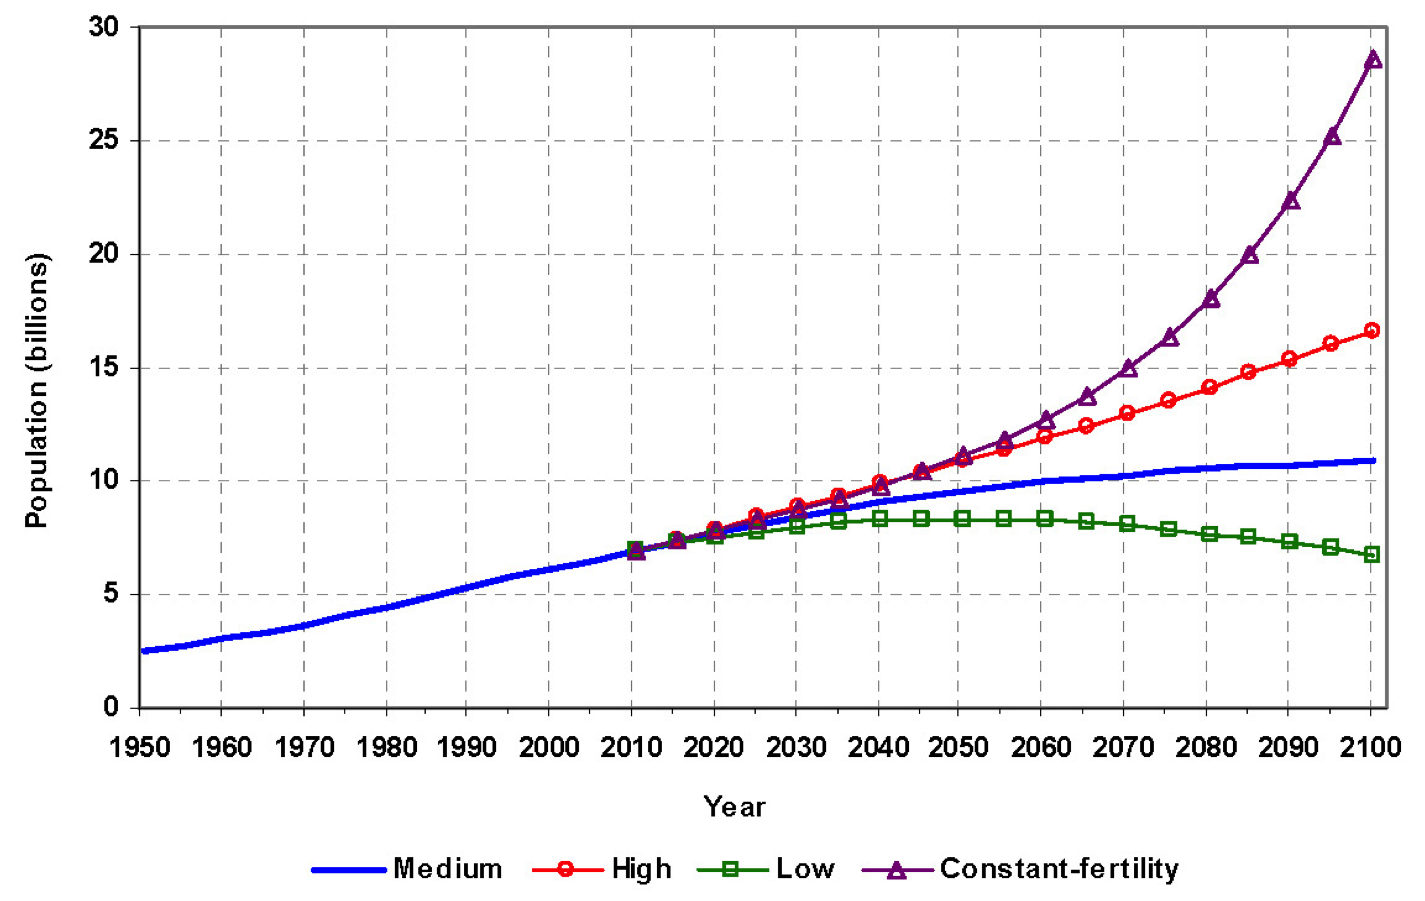
\includegraphics[width=\linewidth]{human-growth-projection.png}}
    \end{adjustwidth}
    \note[item]{A 2014 paper from UW researches predicts 11 billion by 2100
        (= medium projection from U.N.)}
\end{frame}

\begin{frame}[t]
    \begin{adjustwidth}{-2em}{-1.5em}
        \begin{itemize}
            \item What is the definition of replacement rate?

                \nbox{Fertility rate for zero population growth (i.e.,
                    $\popgrowthratediscrete{} = 1$ or $\popgrowthrate{} = 0$).}

                \vspace{1.2cm}
            \item Why isn't the replacement rate 2.0?

                \nbox{Even when survivorship is extremely high, some
                    individuals die before reproducing.}

                \vspace{1cm}
            \item Why is the replacement rate higher in developing countries
                versus industrialized countries?

                \nbox{Higher mortality rates. 2.5-3.3 is a typical range.}
        \end{itemize}
    \end{adjustwidth}
\end{frame}

\clickerslide{
\begin{frame}
    \begin{clickerquestion}
        \item If average global fertility in humans is 2.1 from now until 2050,
            by 2050 the overall growth rate will be 0.47\% per year. Why will
            the population still be increasing?
 
        \begin{clickeroptions}
            \item \clickeranswer{There is an extremely large number of young
                    females in the current population.}
            \item Survivorship will be constant or decrease slightly as the
                planet gets more crowded (and people in developed countries get
                more obese!). 
            \item There are strongly male-biased sex ratios in several
                large-population countries. 
            \item High divorce rates mean that many women are re-marrying and
                starting a second family. 
        \end{clickeroptions}
    \end{clickerquestion}
    \nbox{In less-developed countries, almost half of the population is under
        the age of 25; in least developed countries, more than 60\% of the
        population is under 25.}
\end{frame}
}

\begin{frame}[t]
    \frametitle{Trends in growth rate and fertility}
    \begin{adjustwidth}{-2em}{-1.5em}
        \begin{table}%[htbp]
            \centering
            \begin{tabular}{ L{2cm} C{4cm} C{3cm} }
                & Growth rate/year & Avg.\ fertility (\# of kids/female) \\
                \hline
                1965--70: & 2.04\% & 4.9 \\[2ex]
                1990--95: & 1.46\% & 3.0 \\[2ex]
                2000--05: & 1.2\%  & 2.6 \\[2ex]
                2014:     & 1.12\% & 2.3 \\
            \end{tabular}
        \end{table}

        \vspace{4mm}
        We are currently adding $\approx$77 million people/year \ldots where?

        \nbox{1/2 of current growth is in just 6 countries: India, China,
            Pakistan, Nigeria, Bangladesh, and Indonesia. Many African
            countries are rapidly growing too.}
    \end{adjustwidth}
\end{frame}

\begin{frame}[t]
    \begin{adjustwidth}{-2em}{-1.5em}
        \vspace{-3mm}
        \centering{
            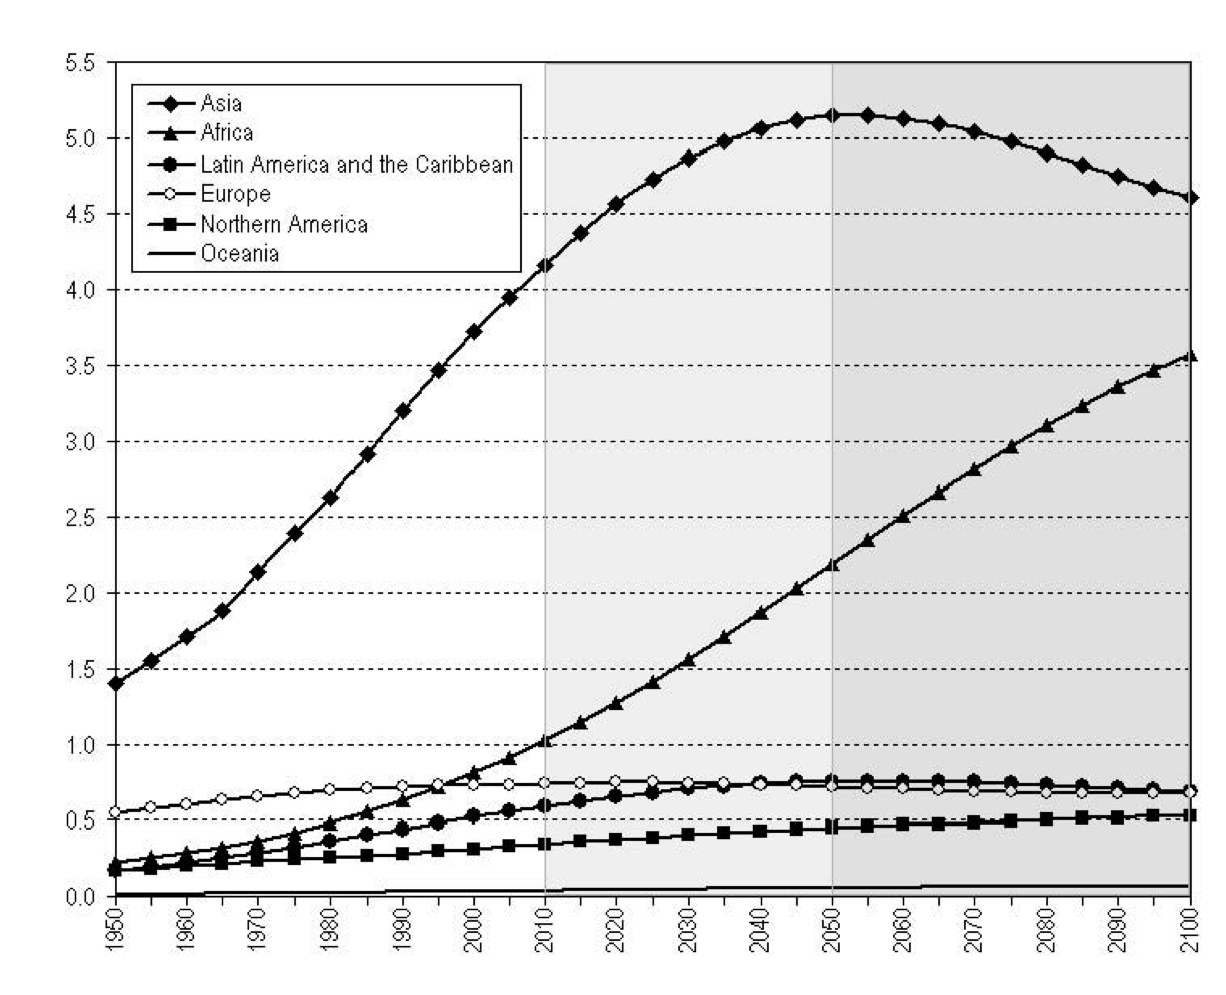
\includegraphics[height=0.9\textheight]{human-growth-projections-regional.png}}

        \vspace{-2mm}
    \nbox{\tiny U.N.\ estimates that in least developed countries, only 38\% of
        women have access to modern contraception}
    \nbox{\tiny UW team predicts 4 billion people in Africa (not 3.6) by 2100.}
    \end{adjustwidth}
\end{frame}

\begin{frame}[t]
    \begin{adjustwidth}{-2em}{-1.5em}
        What conditions contribute to fertility rates, and why?

        \begin{itemize}
            \item Income

                \nbox{As income increases, fertility decreases; higher
                    investment per kid, higher survivorship}

                \vspace{2mm}
            \item Lifespan/child mortality

                \nbox{As child mortality decreases, fertility decreases; when
                    survivorship of kids is higher, can have fewer and invest
                    more in each one}

                \vspace{2mm}
            \item Women's rights (education; access to birth control)

                \nbox{More women's rights, lower fertility; women control and
                    delay reproduction and invest more per kid.}

                \vspace{2mm}
            \item Religious beliefs

                \nbox{Fewer restrictions on contraception, lower fertility}
        \end{itemize}
    \end{adjustwidth}
\end{frame}

% \begin{frame}[t]
%     \begin{adjustwidth}{-2em}{-1.5em}
%         Role of emigration/immigration

%         \begin{itemize}
%             \item Will all the people born in developing countries stay in
%                 developing countries?

%             \vspace{6mm}
%             \item 2004 Pew Hispanic Center survey in Mexico: If you could,
%                 would you emigrate to the United States?

%                 \vspace{4mm}
%                 \begin{itemize}
%                     \item 40\% yes $\times$ 109 million = \cmask{43.6 million}
%                 \end{itemize}

%         \end{itemize}
%     \end{adjustwidth}
% \end{frame}

\begin{frame}[t]
    \begin{adjustwidth}{-2em}{-1.5em}
        In terms of biological impact of humans, the two key factors are:

        \uncover<2->{
        \begin{enumerate}
            \item Number of people (population size)
            
                \vspace{2mm}
            \item Resources used per person
        \end{enumerate}
        }

        \uncover<3->{
        Currently, what is the relationship between these two factors?

        \nbox{Inverse---wealthy countries have low growth but
            disproportionately high resource use.}
        }

        \uncover<4->{
        \vspace{3cm}
        Change is opportunity!
        }
    \end{adjustwidth}
\end{frame}

\section[Fitness trade-offs and life histories]{How do fitness trade-offs
    affect the evolution of life histories?}

\begin{frame}[t]
    \begin{adjustwidth}{-2em}{-1.5em}

        \vspace{-5mm}
        \begin{columns}[t]

            \column{0.64\linewidth}

            How do fitness trade-offs affect the evolution of life histories?
            
            \vspace{4mm}
            Experiment on side-blotched lizards:

            \uncover<2->{
            \begin{enumerate}
                \item Remove yolk from eggs

                    \nbox{Lower investment (smaller young)}

                    \vspace{3mm}
                \item Remove all bu 2--3 eggs

                    \nbox{High investment (larger young)}
            \end{enumerate}
            }

            \column{0.35\linewidth}

            \begin{flushright}
            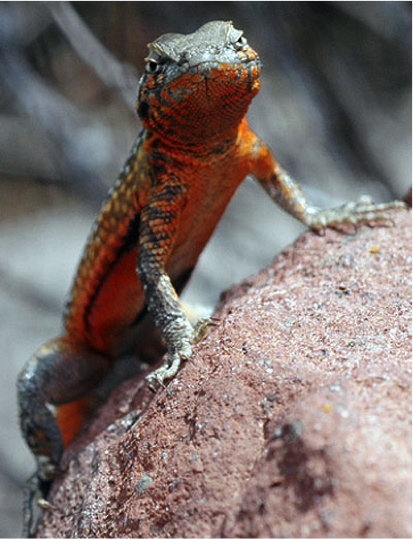
\includegraphics[width=0.85\columnwidth]{uta.png}
            \end{flushright}

        \end{columns}

        \uncover<2->{

        \begin{enumerate}
            \addtocounter{enumi}{2}
            \item Sham operation

                \nbox{Control for operation}
        \end{enumerate}

        In terms of maternal investment per offspring, what does each treatment
        group represent?
        }
    \end{adjustwidth}
\end{frame}

\begin{frame}[t]
    \begin{adjustwidth}{-2em}{-1.5em}
        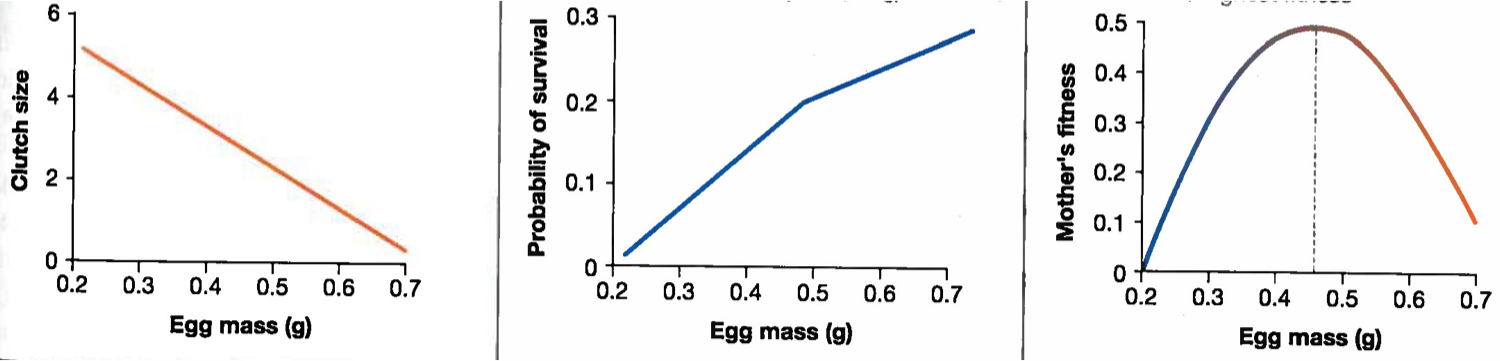
\includegraphics[width=\linewidth]{uta-egg-mass.png}

        \begin{enumerate}
            \item What is the relationship between clutch size and egg size?

                \nbox{Negative---as egg size increases, clutch size decreases}

                \vspace{5mm}
            \item What is the relationship between egg size and offspring
                survival?

                \nbox{Positive---as eggs size increases, survivorship
                    increases}

                \vspace{5mm}
            \item Did mothers that laid large eggs or small eggs have optimal
                fitness?

                \nbox{No, mothers that laid intermediate-sized eggs had optimal
                    fitness}
        \end{enumerate}
    \end{adjustwidth}
\end{frame}

\clickerslide{
\begin{frame}
    \begin{clickerquestion}
        \item These results are evidence for which of the following patterns? 
 
        \begin{clickeroptions}
            \item Disruptive selection
            \item \clickeranswer{Fitness trade-offs}
            \item Directional selection
            \item \clickeranswer{Stabilizing selection}
        \end{clickeroptions}
    \end{clickerquestion}
\end{frame}
}

\clickerslide{
\begin{frame}
    \begin{clickerquestion}
        \item On the south side of Chicago, lifespan in humans is extremely
            low due to poor nutrition, high violence, and inadequate medical
            care. Because education levels are low and unemployment is high,
            men are seldom able to invest in offspring. According to life
            history theory, which of the following is a logical consequence? 
 
        \begin{clickeroptions}
            \item Mothers do not care for their children. 
            \item Male-male competition is intense. 
            \item \clickeranswer{There are many unwed, teenaged mothers.}
            \item Average birthweight is extremely high. 
        \end{clickeroptions}
    \end{clickerquestion}
\end{frame}
}

\end{document}

\clickerslide{
\begin{frame}
    \begin{clickerquestion}
        \item 
        \begin{clickeroptions}
            \item 
            \item 
            \item 
            \item 
        \end{clickeroptions}
    \end{clickerquestion}
\end{frame}
}

\clickerpost{
{
\usebackgroundtemplate{\includegraphics[page=17,width=\paperwidth]{./24-Radiation-extinction.pdf}}
\begin{frame}[t,plain]
    \begin{adjustwidth}{-2em}{-1.5em}
        \cmask{Answer: 3}
    \end{adjustwidth}
\end{frame}
}
}

